\documentclass[a4paper,12pt]{scrartcl}
\usepackage[utf8x]{inputenc}
\usepackage[T1]{fontenc} % avec T1 comme option  d'encodage c'est ben mieux, surtout pour taper du français.
%\usepackage{lmodern,textcomp} % fortement conseillé pour les pdf. On peut mettre autre chose : kpfonts, fourier,...
\usepackage[french]{babel} %Sans ça les guillemets, amarchpo
\usepackage{amsmath}
\usepackage{multicol}
\usepackage{amssymb}
\usepackage{tkz-tab}
\usepackage{exercice_sheet}

%\trait
%\section*{}
%\exo{}
%\question{}
%\subquestion{}

\date{}


% Title Page
\title{Cours \og statistiques à 2 variables \fg{}, corrigé des exercices}

\author{Mathématiques}

\begin{document}

\maketitle

\exo{Exemple de sujet d'examen}

\question{Compléter le tableau:}

\begin{tabular}{@{}|l|l|l|l|l|l|@{}}
\toprule
\textbf{Nombre de sinistres $x_i$} & \textbf{0} & \textbf{1} & \textbf{2} & \textbf{3} & \textbf{4} \\ \midrule
\textbf{Effectifs : $n_i$} & 1345 & 508 & 228 & 78 & 35 \\ \midrule
\textbf{$y_i= \ln n_i$} & 7,20 & 6,23 & 5,43 & 4,36 & 3,56 \\ \bottomrule
\end{tabular}

\question{Coefficient de corrélation.}

Cela se fait à la calculatrice, et on trouve 0,999. On en conclut que la corrélation entre deux variables est bonne et qu'une régression linéaire est pertinente.

\question{Droite de régression.}

On trouve $a = -0.92$ et $b = 7.19$.

\question{2ème année uniquement}

La régression linéaire trouvée question précédente permet d'écrire $y = -0.92x + 7.19$. Or, $y = \ln(n)$.

On peut donc écrire $\ln(n) = -0.92x + 7.19$. On prend l'exponentielle à droite et à gauche: $e^{\ln(n)} = e^{-0.92x + 7.19} \Leftrightarrow n = e^{-0.92x + 7.19}$.

On rappelle que $e^{a+b} = e^a \times e^b$.

Donc: $n = e^{-0.92x} \times e^{7.19}$. $e^{7.19} \approx 1325.4$

On peut donc écrire $n = 1325.4 \times e^{-0.9x}$.

On a bien écrit $n$ sous la forme voulue avec $k = 1325.4$ et $\lambda = -0.9$.

\question{Estimation}

Il suffit d'évaluer le résultat précédent pour $x = 6$: $1325.4 \times e^{-0.9 \times 6} = 5.98$ que l'on arrondit à 6. 

On peut donc estimer qu'il y a 6 véhicules qui ont eu 6 accidents lors de la première année de circulation.

\exo{Fioul}

\question{Nuage de points}

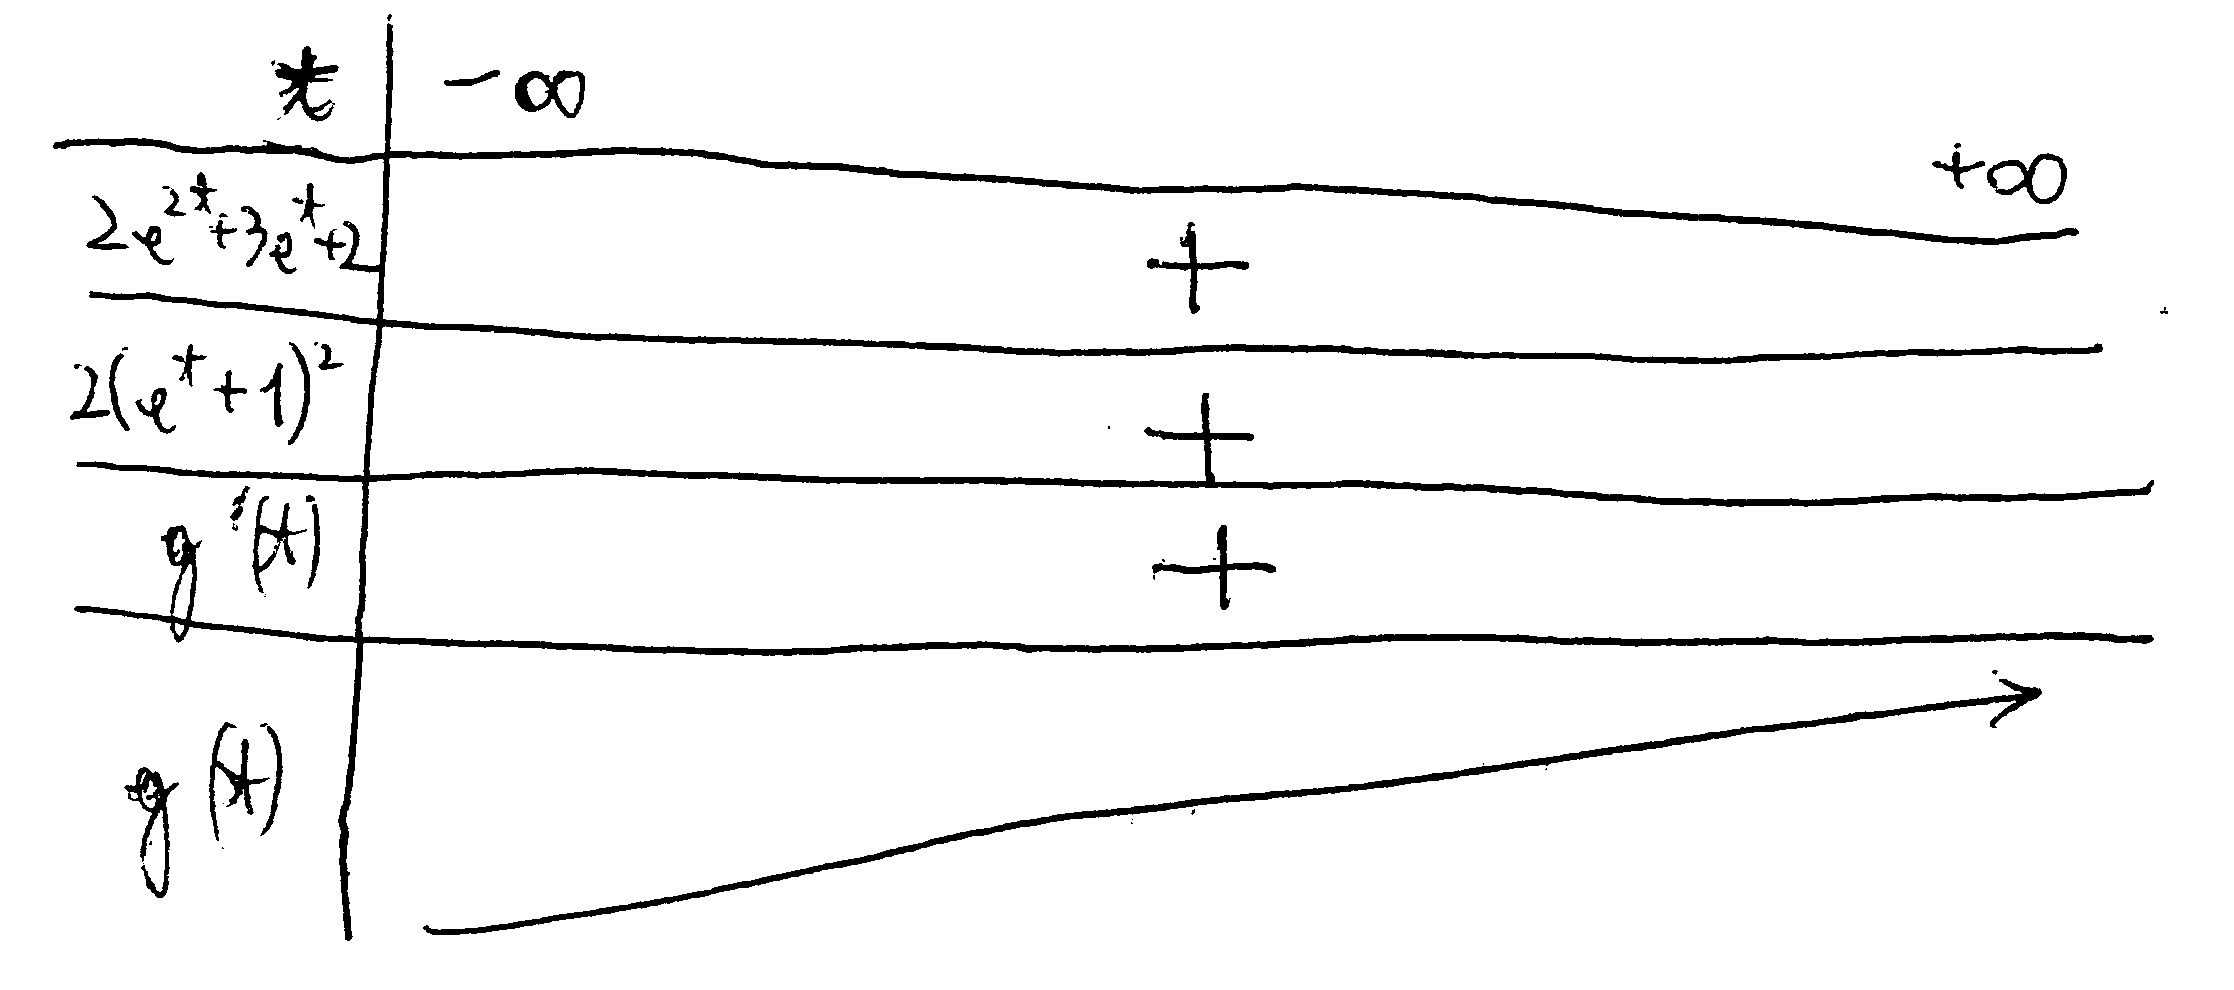
\includegraphics[width=1\textwidth]{pics/1.pdf}

\question{$G_1$ et $G_2$}

$G_1$ a pour abscisse $x_{G_1} = \dfrac{-11-6-3}{3} \approx -6.67$ et pour ordonnée $y_{G_1} = \dfrac{510+400+350}{3} = 420$.

On a donc $G_1(-6.67;420)$.

De la même manière, on trouve $G_2(4.67;240)$.

\question{}

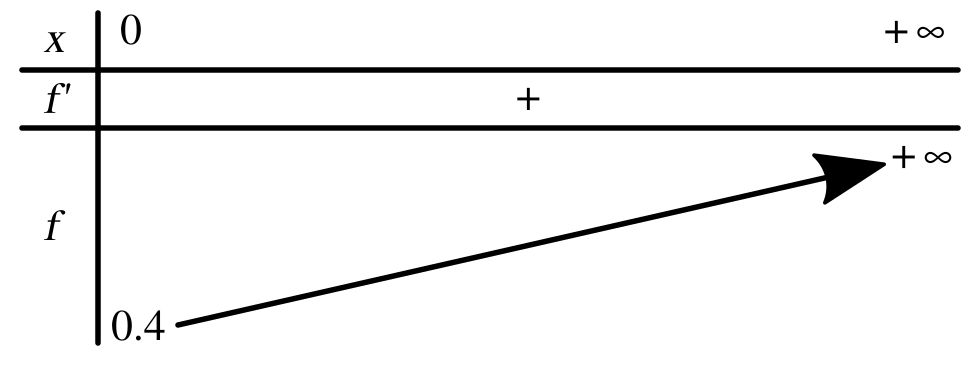
\includegraphics[width=1\textwidth]{pics/2.pdf}

\question{Lecture graphique}

\subquestion{}
On constate sur le graphe qu'une consommation de 250L correspond à une température de 4°C.

\subquestion{}
De la même façon, pour une température de 12°C, on aura une consommation de 125L environ.

\trait

\end{document}
